\newpage
\section{TGGs in action}
\genHeader
\label{sect:TGGs_in_Action}

In order to run our TGG, it first needs to have something tangible to work with. We need to create an instance model\footnote{Refer to Part II, Section 3 for
review} of either one of our language metamodels, which can then be transformed into an instance model of the \emph{other} language (i.e., peform a forward or
backwards transformation). Since dictionaries are a much simpler structure, let's start with the backwards transformation, \texttt{dictionary} to
\texttt{LearningBox}.

\begin{itemize}

\item[$\blacktriangleright$] Navigate to \texttt{Dictionary\-Language/model/} and open \texttt{DictionaryLanguage.ecore}. Create a new
dynamic instance of a \texttt{Dictionary} named \texttt{target.xmi}. Don't quickly press \texttt{enter}! Make sure you save it under
\texttt{Learn\-ing\-Box\-To\-Dictionary\-In\-te\-gra\-tion/in\-stan\-ces/} (Fig.~\ref{fig:create_instance_dict}).

\begin{figure}[htbp]
\begin{center}
  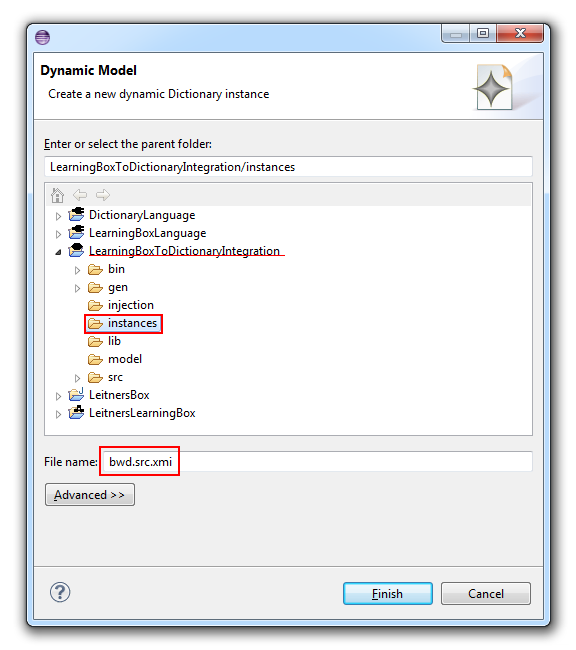
\includegraphics[width=0.8\textwidth]{eclipse_dictionaryInstance}
  \caption{Create a dynamic instance of \texttt{Dictionary}}
  \label{fig:create_instance_dict}
\end{center}
\end{figure}

\item[$\blacktriangleright$] Open \texttt{target.xmi}, and edit the \texttt{Dictionary} properties by setting \texttt{Title} to \texttt{English Numbers}.

\item[$\blacktriangleright$] Create two child \texttt{Entry} objects. Remember the format we constructed? Set \texttt{Content} of the first to \texttt{one :
eins} and its \texttt{Level} as \texttt{beginner}. Set the second with \texttt{eleven : elf} and \texttt{advanced} (Fig.~\ref{fig:dictionaryxmi}).

\begin{figure}[htbp]
\begin{center}
  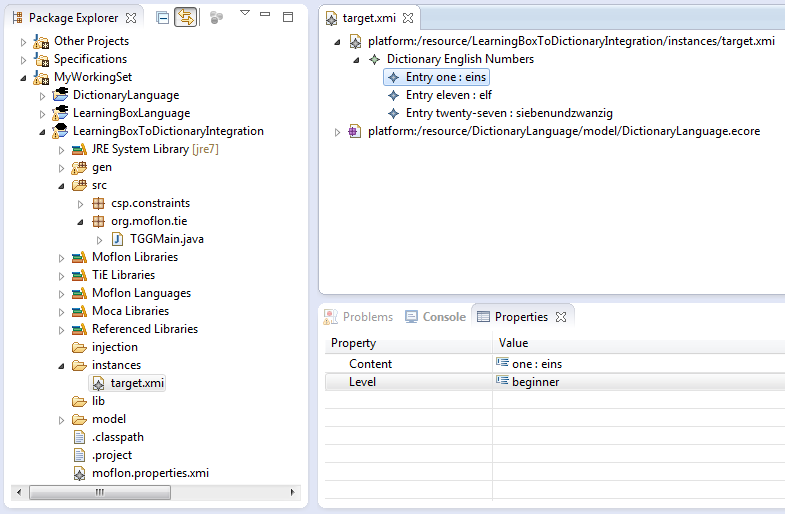
\includegraphics[width=\textwidth]{eclipse_addEntries}
  \caption{Contents of the dictionary}
  \label{fig:dictionaryxmi}
\end{center}
\end{figure}

\item[$\blacktriangleright$] In ``LearningBox\-To\-Dictionary\-In\-te\-gra\-tion\-/src,'' right-click, and navigate to ``Run as\ldots/Java Application'' to run
\texttt{TGGMain} your TGG.

\item[$\blacktriangleright$] In the eMoflon console below the editor, there should  one ``Unable to load instances/source.xmi'' error, followed by a success
message (Fig.~\ref{fig:tggERROR}). Both of these makes sense -- our TGG first attempted a forward transformation but, given that it was missing the source instance,
it was only able to perform a transformation in one direction. Funnily enough however, we actually just created said source file. Since we have our LIST; LIST; and LIST, we
actually created the source graph. If you remember, this was one of our goals of TGG! Given one language, we wanted to be able to derive the other.  This
`error' then becomes an extremely easy fix, where we only need to find the generated instance and rename it.

\begin{figure}[htbp]
\begin{center}
  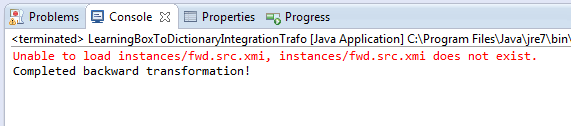
\includegraphics[width=\textwidth]{eclipse_TGGError}
  \caption{comment}
  \label{fig:tggERROR}
\end{center}
\end{figure}

\newpage

\item[$\blacktriangleright$] Refresh the integration's \texttt{instances} folder. There should now be four new \texttt{xmi} files. You created \texttt{target},
\texttt{corr\_BWD} is the correspondence graph between target and source, \texttt{protocol\_BWD} is a listing of the attempted and successful steps taken in the
transformation, and \texttt{target.xmi\_BWD} was the resulting graph. Open this file in the editor.

\item[$\blacktriangleright$] Expand \texttt{box} As you can see, our \texttt{Dictionary} has been translated backward to a \texttt{Box} with the same name
(\texttt{English Numbers}) and containing three \texttt{Par\-ti\-tions} (as specified in \texttt{Box\-To\-Dictionary\-Rule}) (Fig.~\ref{fig:derivedBOX}). The three
\texttt{Entry} objects have been translated to \texttt{Card} objects as specified in \texttt{CartToEntryRule}. The \texttt{face} and the \texttt{back} of the \texttt{Card}s are consistent with the \texttt{content}
of the corresponding \texttt{Entry}, e.g. \texttt{card.face = ``Question : one''} and \texttt{card.back = ``Answer : eins''}. The indices of the partitions
containing the cards are also consistent with the level of the entry, i.e., \texttt{0} for \texttt{beginner}, and \texttt{1} for \texttt{advanced}. \update
mention how the constraints came into play

\begin{figure}[htbp]
\begin{center}
  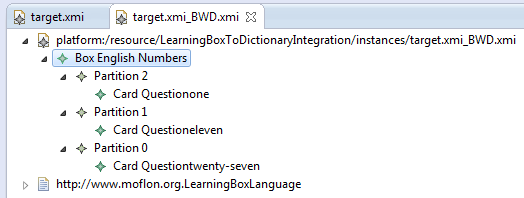
\includegraphics[width=\textwidth]{eclipse_TGGRuleBuiltBOX}
  \caption{our created box}
  \label{fig:derivedBOX}
\end{center}
\end{figure}


mention the graph viewer here! Reemmber the graph view? Its a useful tool, especially with TGGs! Drag and drop \texttt{Box English Numbers} into the graph
viewer. You can see how the partitions are connected via link variables, and you can see which partition contains which card. (Fig.~\ref{fig:graphViewBox}) You
could do this for \texttt{Dictionary} as well, but you'll only have a simple tree graph, with three long lines connecting each entry to the dictionary.

\begin{figure}[htbp]
\begin{center}
  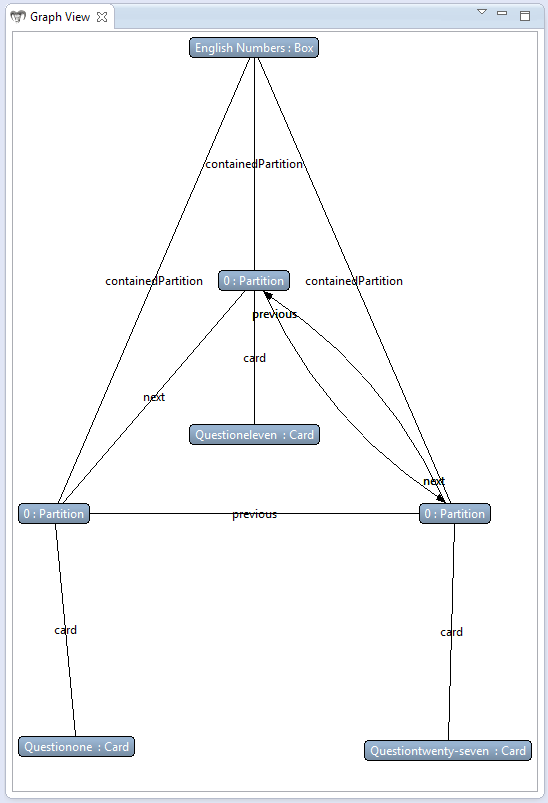
\includegraphics[width=0.8\textwidth]{eclipse_EngNumBoxGraphView}
  \caption{dat graph view. hmmmm.}
  \label{fig:graphViewBox}
\end{center}
\end{figure}


\vspace{0.5cm}

Congratulations! You have successfully performed your first \emph{backward} transformation from your target model (dictionary) to your source (Learning box)
using TGGs! To show that the transformation is actually bidirectional however, lets edit the source model (thus resolving the error from above) and transform it
\emph{forward} to a new target model:


\item[$\blacktriangleright$] Make a copy of \texttt{target.xmi\_BWD.xmi} (the result of the backward transformation)
and rename it to \texttt{source.xmi}.
  
\item[$\blacktriangleright$] Open \texttt{source.xmi} and create some new \texttt{Card} objects in the \texttt{Partition}s (e.g., create a new \texttt{Card}
with \texttt{Card.face = ``Question : two''}, \texttt{Card.back = ``Answer : zwei''} in \texttt{Partition 0}).

\item[$\blacktriangleright$] Run the \texttt{TGGMain.java} again by pressing the green ``Run As\ldots'' icon on the toolbar. No errors should have appeared. and
inspect the result of the forward transformation, target model \texttt{source.xmi\_FWD.xmi}. explain the different files that were generated? as you can see,
\texttt{target} and \texttt{source.xmi\_FWD.xmi} are the same! They were just created different.

\item[$\blacktriangleright$] Try deleting \texttt{target} and running TGGMain on just your source. you should now get an error saying the backwards
transformation DNE. do you get the same result if you open \texttt{source.xmi\_FWD.xmi}? (yes)

\end{itemize}
